\documentclass[a4paper,12pt]{article}

% don't forget the document class, generally : \documentclass[a4paper,12pt]{article}

\usepackage[utf8]{inputenc}
\usepackage[french]{babel}
\usepackage{graphicx}
\usepackage{gensymb}
\usepackage{amsmath}
\usepackage{float}
\usepackage{scrextend}
\usepackage{caption} 
\usepackage{siunitx}
\usepackage{enumitem}
\usepackage{amsthm}
\usepackage{fancyhdr}
\usepackage{amssymb}
\usepackage{wrapfig}
\usepackage{geometry}
\usepackage{standalone}
\usepackage{import}
\usepackage[usenames, dvipsnames]{color}

 \usepackage{biblatex} % manages bibliography and references
\addbibresource{sample.bib}


\geometry{hmargin=1in, vmargin=1in}

 \newenvironment{absolutelynopagebreak}
 {\par\nobreak\vfil\penalty0\vfilneg
 \vtop\bgroup}
 {\par\xdef\tpd{\the\prevdepth}\egroup
 \prevdepth=\tpd}
 
 \pagestyle{fancy}                        
\fancyhf{}                               
\fancyhf[HL]{Application des maths}                
\fancyhf[HR]{Géométrie euclidienne}             
\fancyhf[FC]{\thepage/\pageref{Lastpage}}
 
\newtheorem{definition}{Définition}[section]
\newtheorem{theorem}{Théorème}
\newtheorem{corollary}{Corollaire}[theorem]
\newtheorem{lemma}[theorem]{Lemme}
\newtheorem*{hyp}{Hypothèse}
\newtheorem*{concl}{Conclusion}
\newtheorem*{remark}{Remarque}

\captionsetup{format=default,labelformat=simple,labelsep=colon,
justification=justified,font={sf,small},labelfont=bf,
textfont=default} 



\begin{document}

\pagebreak
\subsection{Deuxième cas d'isométrie des triangles}
\begin{theorem}
Deux triangles qui ont respectivement un côté et les angles adjacents isométriques sont isométriques.
\end{theorem}
\begin{hyp}
$a_1 \equiv a_2$, $\beta_1 \equiv \beta_2$ et $\gamma_1 \equiv \gamma_2$
\end{hyp}
\begin{concl}
$b_1 \equiv b_2$, $c_1 \equiv c_2$ et que $\alpha_1 \equiv \alpha_2$
\end{concl}
\begin{proof}
Considérons deux triangles $\triangle a_1b_1c_1$ et $\triangle a_2b_2c_2$. Nous avons reporté le côté $c_2$ sur le côté $c_1$. alors, il y a trois possibilités:
\begin{figure}[H]
    \centering
    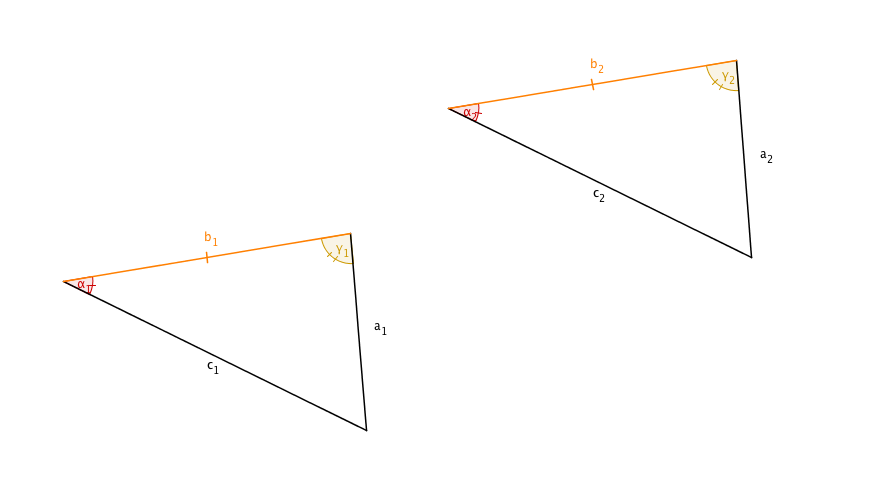
\includegraphics[scale=0.45]{theorems/isom2/cas2.png}
\end{figure}
\begin{enumerate}
\item $c_1 = c_2$, alors les deux triangles sont isométriques (axiome III)
\item $c_1<c_2$
\item $c_1>c_2$
\end{enumerate}

\pagebreak
Dans le deuxième et troisième cas, on forme le triangle $\triangle b_1b_3c_2'$. Ce triangle est isométrique au triangle $\triangle a_2b_2c_2$, car ils ont en commun un angle compris entre deux côtés isométriques. Par conséquent, $\gamma_2\equiv \gamma_3$, donc $\gamma_1$ et $\gamma_3$ sont confondus, d est nul et $c_1\equiv c_2$. On en revient donc au premier cas: les deux triangles $\triangle a_1b_1c_1$ et $\triangle a_2b_2c_2$ sont isométriques grâce au premier cas d'isométrie des triangles.


\begin{figure}[H]
    \centering
    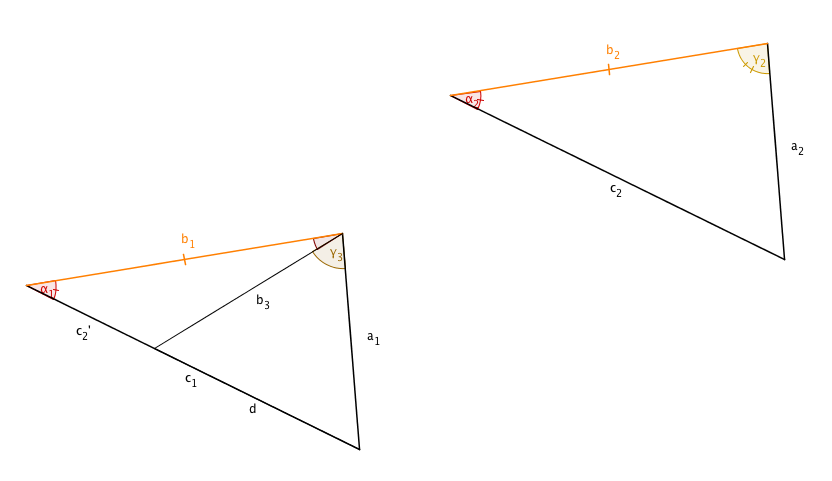
\includegraphics[scale=0.6]{theorems/isom2/Cas2_2.png}
\end{figure}



\end{proof}

\end{document}
